\documentclass[Royal,times,sageh]{sagej}

\usepackage{moreverb,url,natbib, multirow, tabularx}
\usepackage[colorlinks,bookmarksopen,bookmarksnumbered,citecolor=red,urlcolor=red]{hyperref}



% tightlist command for lists without linebreak
\providecommand{\tightlist}{%
  \setlength{\itemsep}{0pt}\setlength{\parskip}{0pt}}



\usepackage{booktabs}
\usepackage{longtable}
\usepackage{array}
\usepackage{multirow}
\usepackage{wrapfig}
\usepackage{float}
\usepackage{colortbl}
\usepackage{pdflscape}
\usepackage{tabu}
\usepackage{threeparttable}
\usepackage{threeparttablex}
\usepackage[normalem]{ulem}
\usepackage{makecell}
\usepackage{xcolor}


\begin{document}


\setcitestyle{aysep={,}}

\title{ActiveCA: an open data product on active transportation episodes
in Canada}

\runninghead{}

\author{Anon1\affilnum{}, Anon2\affilnum{}, Anon3\affilnum{}}

\affiliation{\affilnum{}{}}



\begin{abstract}
This paper describes the data set of the \{ActiveCA\} R data package.
\{ActiveCA\} contains open data products to obtain impedance functions
for active transportation modes in Canada, retrieved from the General
Social Survey collections from 1986 to 2015. The package provides data
tables on walking and cycling episodes, detailing the trip origins,
destinations, and duration of each episode. The origin and destination
categories covers a wide variety of locations, such as home, work or
school, libraries, museums, restaurants, bars, sports centers, health
clinics, place of worship, and others. Addittionally, the package
details the respondent's region characteristics, specifying wheter they
live in a metropolitan area and their province of residency.
\{ActiveCA\} enables users to calculate the average travel time for each
origin-destination combination for each survey year, considering the two
active transportation modes: walking and cycling. For each Census
Metropolitan and Agglomeration Area, we estimated distance-decay curves
(impedance functions) for each destination, transportation mode and
year. The package will continue to expand with contributions from the
authors and the broader community through requests in the future.
\{ActiveCA\} is freely accessible for exploration and download from the
associated Github repository, where the documentation and code involved
in creating and manipulating data and all open data products are
detailed.
\end{abstract}

\keywords{Active; mobility; walking; cycling; travel time; impedance;
transportation; R}

\maketitle

\hypertarget{introduction}{%
\section{Introduction}\label{introduction}}

This paper presents the open data product \{ActiveCA\}. Open data
products (ODPs) are the outcome of a transparent process that transforms
raw data (open or not) into analysis-ready data, in which all stages of
development follow open principles \citep{arribas-bel2021}. ODPs differ
from general open data due to their high utility, added value and open
availability. The product presented in this document is an \texttt{R}
data package that currently consists of processed data tables retrieved
from the Time Use collections of the General Social Surveys (GSS) from
1986 to 2015 \citep{statisticscanada2024}, aimed to obtain impedance
functions for active transportation modes in Canada.

To create this \texttt{R} data package, we collected, cleaned and
processed the Time Use collections from the GSS surveys to make them
ready for analysis. An \texttt{R} data package contains code, data and
documentation in a standardized format that can be installed by
\texttt{R} users via a centralized software repository, such as CRAN
(Comprehensive R Archive Network) and GitHub. Although the GSS surveys
are publicly sourced and managed by Statistic Canada, preparing them for
analysis can be time-consuming, tedious and perhaps not even possible
for those who try, due to a lack of documentation or prior knowledge.

The aim of this paper is to walk readers through the data sets and
invite others to experiment in its uses and applications. \{ActiveCA\}
is freely available on GitHub for all to install and freely use in the
spirit of open and reproducible research. Although \{ActiveCA\} was
designed to obtain impedance functions, we admit and hope that its use
can be adopted in various applications that even go beyond the range of
possibilities we have imagined. Not only the data, but also all the code
documenting the processing methodology is available for consultation and
evaluation in its repository. This package contributes to reducing the
barrier to using the information contained in GSS surveys to provide
data-driven decisions in transportation analysis.

\hypertarget{general-social-survey-gss-collection}{%
\section{General Social Survey (GSS)
collection}\label{general-social-survey-gss-collection}}

Statistics Canada \citeyearpar{statisticscanada2024} conducts GSS
surveys to obtain data on social trends to track changes in Canadians'
living conditions and well-being over time. This survey is used to
understand how citizens spend and manage their time and what factors
contribute to their happiness and stress. Created in 1985, the survey is
part of a series of independent, annual, and cross-sectional surveys.

In addition to the main topic, each GSS cycle includes new content that
addresses emerging and policy-relevant issues. Every five to seven
years, the Time Use Surveys \citep{statisticscanada2022} collect data on
respondents' participation and time spent on a wide range of everyday
activities using a 24-hour retrospective diary, with information on the
location of these activities (e.g.~at home, at work, etc.) and, for
non-personal activities, the people who were present with the respondent
at the time of the activity. In addition, time-use surveys also cover
topics related to leisure time, work-life balance, health, commuting,
culture and sports, and many others.

The most recent time use survey was carried out in 2022
\citep{wray2024}. However, the 2022 dataset has not been fully published
and, because of this, our analysis focused on the surveys from 1986 to
2015 (1986, 1992, 1998, 2005, 2010 and 2015). Time Use surveys are
composed of two data sets, the main one and the episode file, explained
in the following subsections.

\hypertarget{the-main-file}{%
\subsection{The Main File}\label{the-main-file}}

The Main File compiles an large array of aggregated data, summarizing
the answers to the questionnaire and derived variables that summarize
the respondents' time use across different activities, locations, and
social interactions. This file documents the time and duration that
respondents allocate to each activity and location. The Main File
provides a overview of daily routines and social dynamics, not focusing
on individual activity episodes. Additionally, this file categorizes
activities into bigger groups and subcategories, facilitating the data's
analytical utility with additional metrics such as total transit time,
duration spent with household members, and counts of activities and
episodes.

\hypertarget{the-episode-file}{%
\subsection{The Episode File}\label{the-episode-file}}

The Episode File records detailed data for each activity episode
reported by respondents. The entry includes the start and end times,
duration, location, and accompanying social context, informing when and
where activities occurred and with whom. The file distinguishes itself
by focusing on individual episodes rather than respondents, with the
data structured around the numerous activity instances that compose a
day of the respondent. Although respondent-specific characteristics are
not included within the Episode File, it is possible to link the Main
File and the Episode File by using an identifiable variable present in
both data sets.

\hypertarget{descriptive-statistics}{%
\section{Descriptive statistics}\label{descriptive-statistics}}

For each year available from the Time Use surveys, we reviewed the
episode files to identify cases with activities listed as walking or
cycling and selected the activities immediately before and after the
mobility episode. The \{ActiveCA\} package includes all 21748 episodes
that recorded walking or cycling as a mode of transportation, with trip
durations ranging from 0 to 900 minutes. Among the analyses possible
with this package, Table \ref{tab:table-01} presents descriptive
statistics on walking and cycling trips between 1986 and 2015, including
metrics such as the count of recorded trips (count), and measures of
trip duration in minutes: maximum (max), mean, median, and minimum
(min). The 1986 survey did not include bicycle trips.

\begingroup\fontsize{10}{12}\selectfont

\begin{longtable}[t]{>{}llcccccc}
\caption{\label{tab:table-01}\label{tab:table-01}Descriptive statistics for episodes with active transport records}\\
\toprule
\multicolumn{2}{c}{ } & \multicolumn{6}{c}{Year} \\
\cmidrule(l{3pt}r{3pt}){3-8}
Mode & Statistic & 1986 & 1992 & 1998 & 2005 & 2010 & 2015\\
\midrule
 & count & 4347 & 1500 & 1670 & 5533 & 4379 & 3251\\
\nopagebreak
 & max & 660 & 300 & 255 & 515 & 480 & 900\\
\nopagebreak
 & mean & 21 & 19 & 11 & 12 & 12 & 17\\
\nopagebreak
 & median & 10 & 10 & 5 & 10 & 8 & 10\\
\nopagebreak
\multirow[t]{-5}{*}{\raggedright\arraybackslash \textbf{Walking}} & min & 1 & 1 & 1 & 0 & 0 & 5\\
\cmidrule{1-8}\pagebreak[0]
 & count & NA & 135 & 119 & 333 & 236 & 245\\
\nopagebreak
 & max & NA & 240 & 90 & 180 & 153 & 120\\
\nopagebreak
 & mean & NA & 31 & 21 & 19 & 21 & 24\\
\nopagebreak
 & median & NA & 20 & 15 & 15 & 15 & 15\\
\nopagebreak
\multirow[t]{-5}{*}{\raggedright\arraybackslash \textbf{Cycling}} & min & NA & 5 & 2 & 1 & 1 & 5\\
\bottomrule
\end{longtable}
\endgroup{}

Table \ref{tab:table-01} shows that the median values for walking trips
range between 5 and 10 minutes, while cycling trips have a consistent
median of 15 minutes since 1998. The table also highlights very high
maximum values, particularly for walking trips, with recorded episodes
exceeding 4 hours in all cases.

Table \ref{tab:table-02} and \ref{tab:table-03} provide descriptive
statistics for the two modes of transportation, split by destination
categories, from 1986 to 1998 and from 2005 to 2015, respectively. In
Table \ref{tab:table-02}, one can observed that in 1986 and 1992,
walking trips destined for \texttt{home} had the highest medians.
However, by 1998, the highest medians shifted to trips to
\texttt{work\ or\ school}, a transition that also occurred for cycling
trips between 1992 and 1998. Table \ref{tab:table-03} indicates that the
median duration for trips to \texttt{home} and \texttt{work\ or\ school}
remained at 10 minutes.

\begingroup\fontsize{6}{8}\selectfont

\begin{ThreePartTable}
\begin{TableNotes}
\item \textit{Note: } 
\item * The symbols used in this table represent the following: `Min` denotes the minimum time to reach the destination; `Max` denotes the maximum time to reach the destination; `(\%)` indicates a percentage of the total time to reach the destination; `Med` refers to the median time to reach the destination
\end{TableNotes}
\begin{longtable}[t]{ccccc>{}c|ccc>{}c|cccc}
\caption{\label{tab:table-02}\label{tab:table-02}Comparison of travel statistics by mode and destination: 1986, 1992, 1998}\\
\toprule
\multicolumn{2}{c}{ } & \multicolumn{4}{c}{1986} & \multicolumn{4}{c}{1992} & \multicolumn{4}{c}{1998} \\
\cmidrule(l{3pt}r{3pt}){3-6} \cmidrule(l{3pt}r{3pt}){7-10} \cmidrule(l{3pt}r{3pt}){11-14}
\multicolumn{1}{c}{\textbf{Destination}} & \multicolumn{1}{c}{\textbf{Mode*}} & \multicolumn{1}{c}{\textbf{Min*}} & \multicolumn{1}{c}{\textbf{Med*}} & \multicolumn{1}{c}{\textbf{Max*}} & \multicolumn{1}{c}{\textbf{(\%)*}} & \multicolumn{1}{c}{\textbf{Min}} & \multicolumn{1}{c}{\textbf{Med}} & \multicolumn{1}{c}{\textbf{Max}} & \multicolumn{1}{c}{\textbf{(\%)}} & \multicolumn{1}{c}{\textbf{Min}} & \multicolumn{1}{c}{\textbf{Med}} & \multicolumn{1}{c}{\textbf{Max}} & \multicolumn{1}{c}{\textbf{(\%)}}\\
\midrule
Home &  & NA & NA & NA & NA & 5 & 20 & 240 & 55.6 & 2 & 15.0 & 90 & 52.9\\
Home &  & 1 & 15 & 330 & 46.4 & 1 & 10 & 300 & 59.5 & 1 & 5.0 & 255 & 51.6\\
Other's home & Cycling & NA & NA & NA & NA & 5 & 10 & 145 & 18.5 & 2 & 10.0 & 80 & 17.6\\
Other's home & Walking & 1 & 10 & 660 & 42.3 & 1 & 5 & 135 & 21.3 & 1 & 5.0 & 120 & 28.1\\
Work or school &  & NA & NA & NA & NA & 5 & 15 & 45 & 25.9 & 5 & 20.0 & 75 & 29.4\\
\addlinespace
Work or school &  & 1 & 10 & 450 & 11.3 & 2 & 10 & 60 & 19.2 & 1 & 6.5 & 75 & 20.4\\
\bottomrule
\insertTableNotes
\end{longtable}
\end{ThreePartTable}
\endgroup{}

\begingroup\fontsize{6}{8}\selectfont

\begin{ThreePartTable}
\begin{TableNotes}
\item \textit{Note: } 
\item * The symbols used in this table represent the following: `Min` denotes the minimum time to reach the destination; `Max` denotes the maximum time to reach the destination; `(\%)` indicates a percentage of the total time to reach the destination; `Med` refers to the median time to reach the destination
\end{TableNotes}
\begin{longtable}[t]{>{\centering\arraybackslash}p{2cm}>{\centering\arraybackslash}p{0.4cm}>{\centering\arraybackslash}p{0.4cm}>{\centering\arraybackslash}p{0.4cm}>{\centering\arraybackslash}p{0.4cm}>{}c|>{\centering\arraybackslash}p{0.4cm}>{\centering\arraybackslash}p{0.4cm}>{\centering\arraybackslash}p{0.4cm}>{}c|>{\centering\arraybackslash}p{0.4cm}>{\centering\arraybackslash}p{0.4cm}>{\centering\arraybackslash}p{0.4cm}>{\centering\arraybackslash}p{0.4cm}}
\caption{\label{tab:table-03}\label{tab:table-03}Comparison of travel statistics by mode and destination: 2005, 2010, 2015}\\
\toprule
\multicolumn{2}{c}{ } & \multicolumn{4}{c}{2005} & \multicolumn{4}{c}{2010} & \multicolumn{4}{c}{2015} \\
\cmidrule(l{3pt}r{3pt}){3-6} \cmidrule(l{3pt}r{3pt}){7-10} \cmidrule(l{3pt}r{3pt}){11-14}
\multicolumn{1}{>{\centering\arraybackslash}p{2cm}}{\textbf{Destination}} & \multicolumn{1}{>{\centering\arraybackslash}p{0.4cm}}{\textbf{Mode*}} & \multicolumn{1}{>{\centering\arraybackslash}p{0.4cm}}{\textbf{Min*}} & \multicolumn{1}{>{\centering\arraybackslash}p{0.4cm}}{\textbf{Med*}} & \multicolumn{1}{>{\centering\arraybackslash}p{0.4cm}}{\textbf{Max*}} & \multicolumn{1}{>{\centering\arraybackslash}p{0.4cm}}{\textbf{(\%)*}} & \multicolumn{1}{>{\centering\arraybackslash}p{0.4cm}}{\textbf{Min}} & \multicolumn{1}{>{\centering\arraybackslash}p{0.4cm}}{\textbf{Med}} & \multicolumn{1}{>{\centering\arraybackslash}p{0.4cm}}{\textbf{Max}} & \multicolumn{1}{>{\centering\arraybackslash}p{0.4cm}}{\textbf{(\%)}} & \multicolumn{1}{>{\centering\arraybackslash}p{0.4cm}}{\textbf{Min}} & \multicolumn{1}{>{\centering\arraybackslash}p{0.4cm}}{\textbf{Med}} & \multicolumn{1}{>{\centering\arraybackslash}p{0.4cm}}{\textbf{Max}} & \multicolumn{1}{>{\centering\arraybackslash}p{0.4cm}}{\textbf{(\%)}}\\
\midrule
Business &  & NA & NA & NA & NA & NA & NA & NA & NA & 5 & 10.0 & 30 & 0.2\\
Cultural venues &  & 10 & 12.5 & 15 & 0.6 & 10 & 25 & 30 & 1.3 & 15 & 15.0 & 15 & 0.8\\
Cultural venues & Walking & 5 & 12.5 & 40 & 0.6 & 2 & 10 & 40 & 0.7 & 5 & 10.0 & 40 & 1.5\\
Grocery store & Cycling & 2 & 10.0 & 30 & 10.2 & 5 & 10 & 75 & 8.9 & 5 & 15.0 & 80 & 6.5\\
Grocery store &  & 1 & 10.0 & 90 & 12.5 & 1 & 8 & 105 & 13.2 & 5 & 10.0 & 130 & 11.8\\
\addlinespace
Health clinic &  & NA & NA & NA & NA & NA & NA & NA & NA & 10 & 15.0 & 90 & 2.0\\
Health clinic &  & NA & NA & NA & NA & NA & NA & NA & NA & 5 & 10.0 & 130 & 1.0\\
Home &  & 1 & 15.0 & 180 & 48.9 & 1 & 15 & 135 & 50.4 & 5 & 20.0 & 120 & 46.9\\
Home &  & 0 & 10.0 & 515 & 44.4 & 0 & 10 & 270 & 43.6 & 5 & 10.0 & 900 & 45.3\\
Neighbourhood &  & NA & NA & NA & NA & NA & NA & NA & NA & 10 & 30.0 & 45 & 1.2\\
\addlinespace
Neighbourhood &  & NA & NA & NA & NA & NA & NA & NA & NA & 5 & 10.0 & 60 & 2.1\\
Other's home &  & 1 & 15.0 & 35 & 9.0 & 5 & 10 & 45 & 9.3 & 5 & 15.0 & 40 & 5.3\\
Other's home &  & 1 & 5.0 & 300 & 11.7 & 0 & 5 & 140 & 11.3 & 5 & 10.0 & 120 & 7.3\\
Outdoors &  & 5 & 15.0 & 45 & 6.0 & 3 & 10 & 115 & 3.8 & 15 & 20.0 & 30 & 1.2\\
Outdoors &  & 1 & 5.0 & 295 & 3.6 & 0 & 10 & 480 & 5.2 & 5 & 10.0 & 135 & 2.8\\
\addlinespace
Place of worship &  & 20 & 20.0 & 20 & 0.3 & NA & NA & NA & NA & 15 & 15.0 & 15 & 0.4\\
Place of worship &  & 1 & 10.0 & 30 & 0.8 & 1 & 8 & 60 & 0.9 & 5 & 15.0 & 45 & 1.1\\
Restaurant &  & 5 & 20.0 & 35 & 3.0 & 10 & 15 & 153 & 2.1 & 10 & 17.5 & 60 & 4.1\\
Restaurant &  & 0 & 5.0 & 85 & 9.3 & 1 & 5 & 153 & 10.0 & 5 & 10.0 & 120 & 8.4\\
Sport area &  & NA & NA & NA & NA & NA & NA & NA & NA & 10 & 15.0 & 15 & 2.9\\
\addlinespace
Sport area &  & NA & NA & NA & NA & NA & NA & NA & NA & 5 & 10.0 & 45 & 3.3\\
Work or school &  & 1 & 15.0 & 90 & 21.9 & 1 & 15 & 100 & 24.2 & 5 & 15.0 & 120 & 28.6\\
Work or school &  & 0 & 10.0 & 175 & 17.1 & 0 & 10 & 150 & 15.0 & 5 & 10.0 & 190 & 15.1\\
\bottomrule
\insertTableNotes
\end{longtable}
\end{ThreePartTable}
\endgroup{}

\{ActiveCA\} also enables visual analysis with traditional exploratory
data analysis techniques. Figures \ref{fig:figure-01} and
\ref{fig:figure-02} show walking and cycling trips from 1992 and 2015
through heat maps. These maps use color gradients to represent the
percentage of trips between various origins and destinations, with
darker colors indicating higher percentages and lighter colors
representing less frequent routes. To avoid overwhelming the reader, we
omitted the heat maps for the other years analyzed.

In 1992, walking trips with \texttt{home} as both the origin and
destination made up the majority, accounting for about 30\% of all
walking trips. These trips often involved leisure activities, like short
walks or dog walking. Following this, trips from \texttt{home} to
\texttt{work\ or\ school} comprised 18\% of walking trips. Overall,
\texttt{home} emerged as a crucial hub, either as an origin or
destination, with only 5\% of trips not involving \texttt{home.} By
2015, \texttt{home} remained a significant node, but new locations
distributed the proportion of trips to areas not considered in 1992. In
2015, the highest proportion of trips were from \texttt{home} to
\texttt{work\ or\ school} (12\%) and vice versa (11\%). \texttt{home} to
\texttt{home} accounted for 8\% of trips, and \texttt{grocery\ stores}
became a notable destination for those leaving \texttt{home} (6\%),
surpassing trips to \texttt{other\textquotesingle{}s\ home} (4\%).

\begin{figure}

{\centering 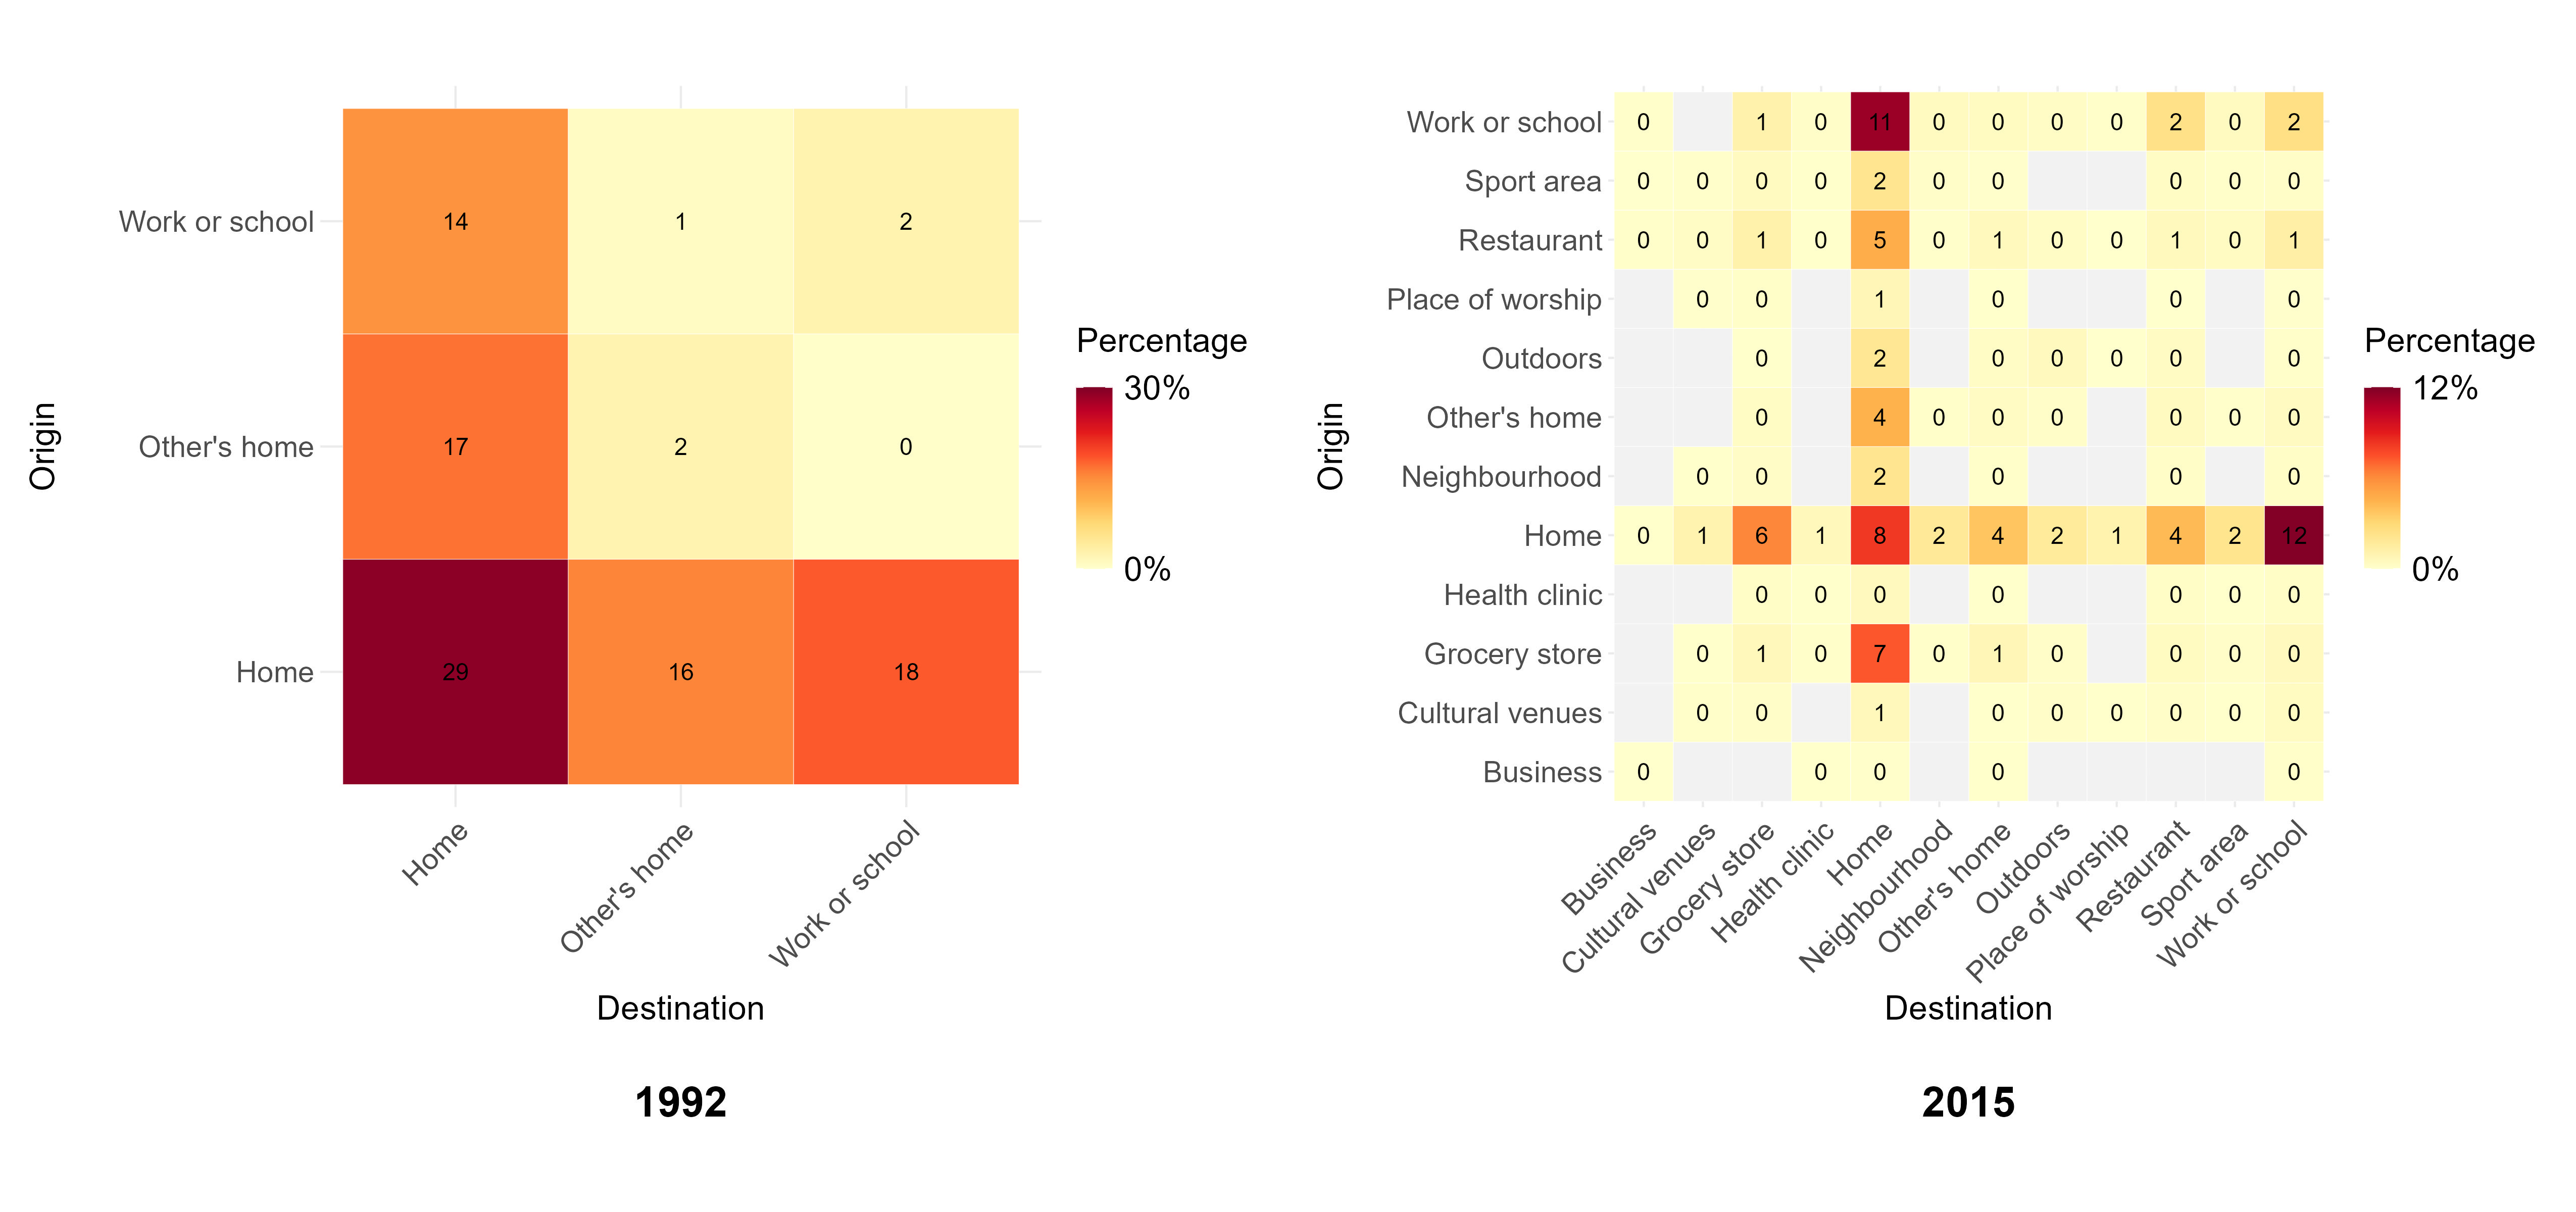
\includegraphics[width=1\linewidth]{Manuscript-figures/walking_hm_fig} 

}

\caption{Percentage of walking Trips Categorized by Origin and Destination}\label{fig:figure-01}
\end{figure}

For cycling trips, Figure \ref{fig:figure-02}, shows that in 1992, when
this mode of transportation was first included as an activity, the
majority of trips were from \texttt{home} to \texttt{work\ or\ school},
accounting for about 25\% of cases. This pattern remained in 2015, with
these trips representing 30\% of the cases. However, a notable change
occurred in \texttt{home} to \texttt{home} trips, which decreased
significantly from 19\% in 1992 to 5\% in 2015.

\begin{figure}

{\centering 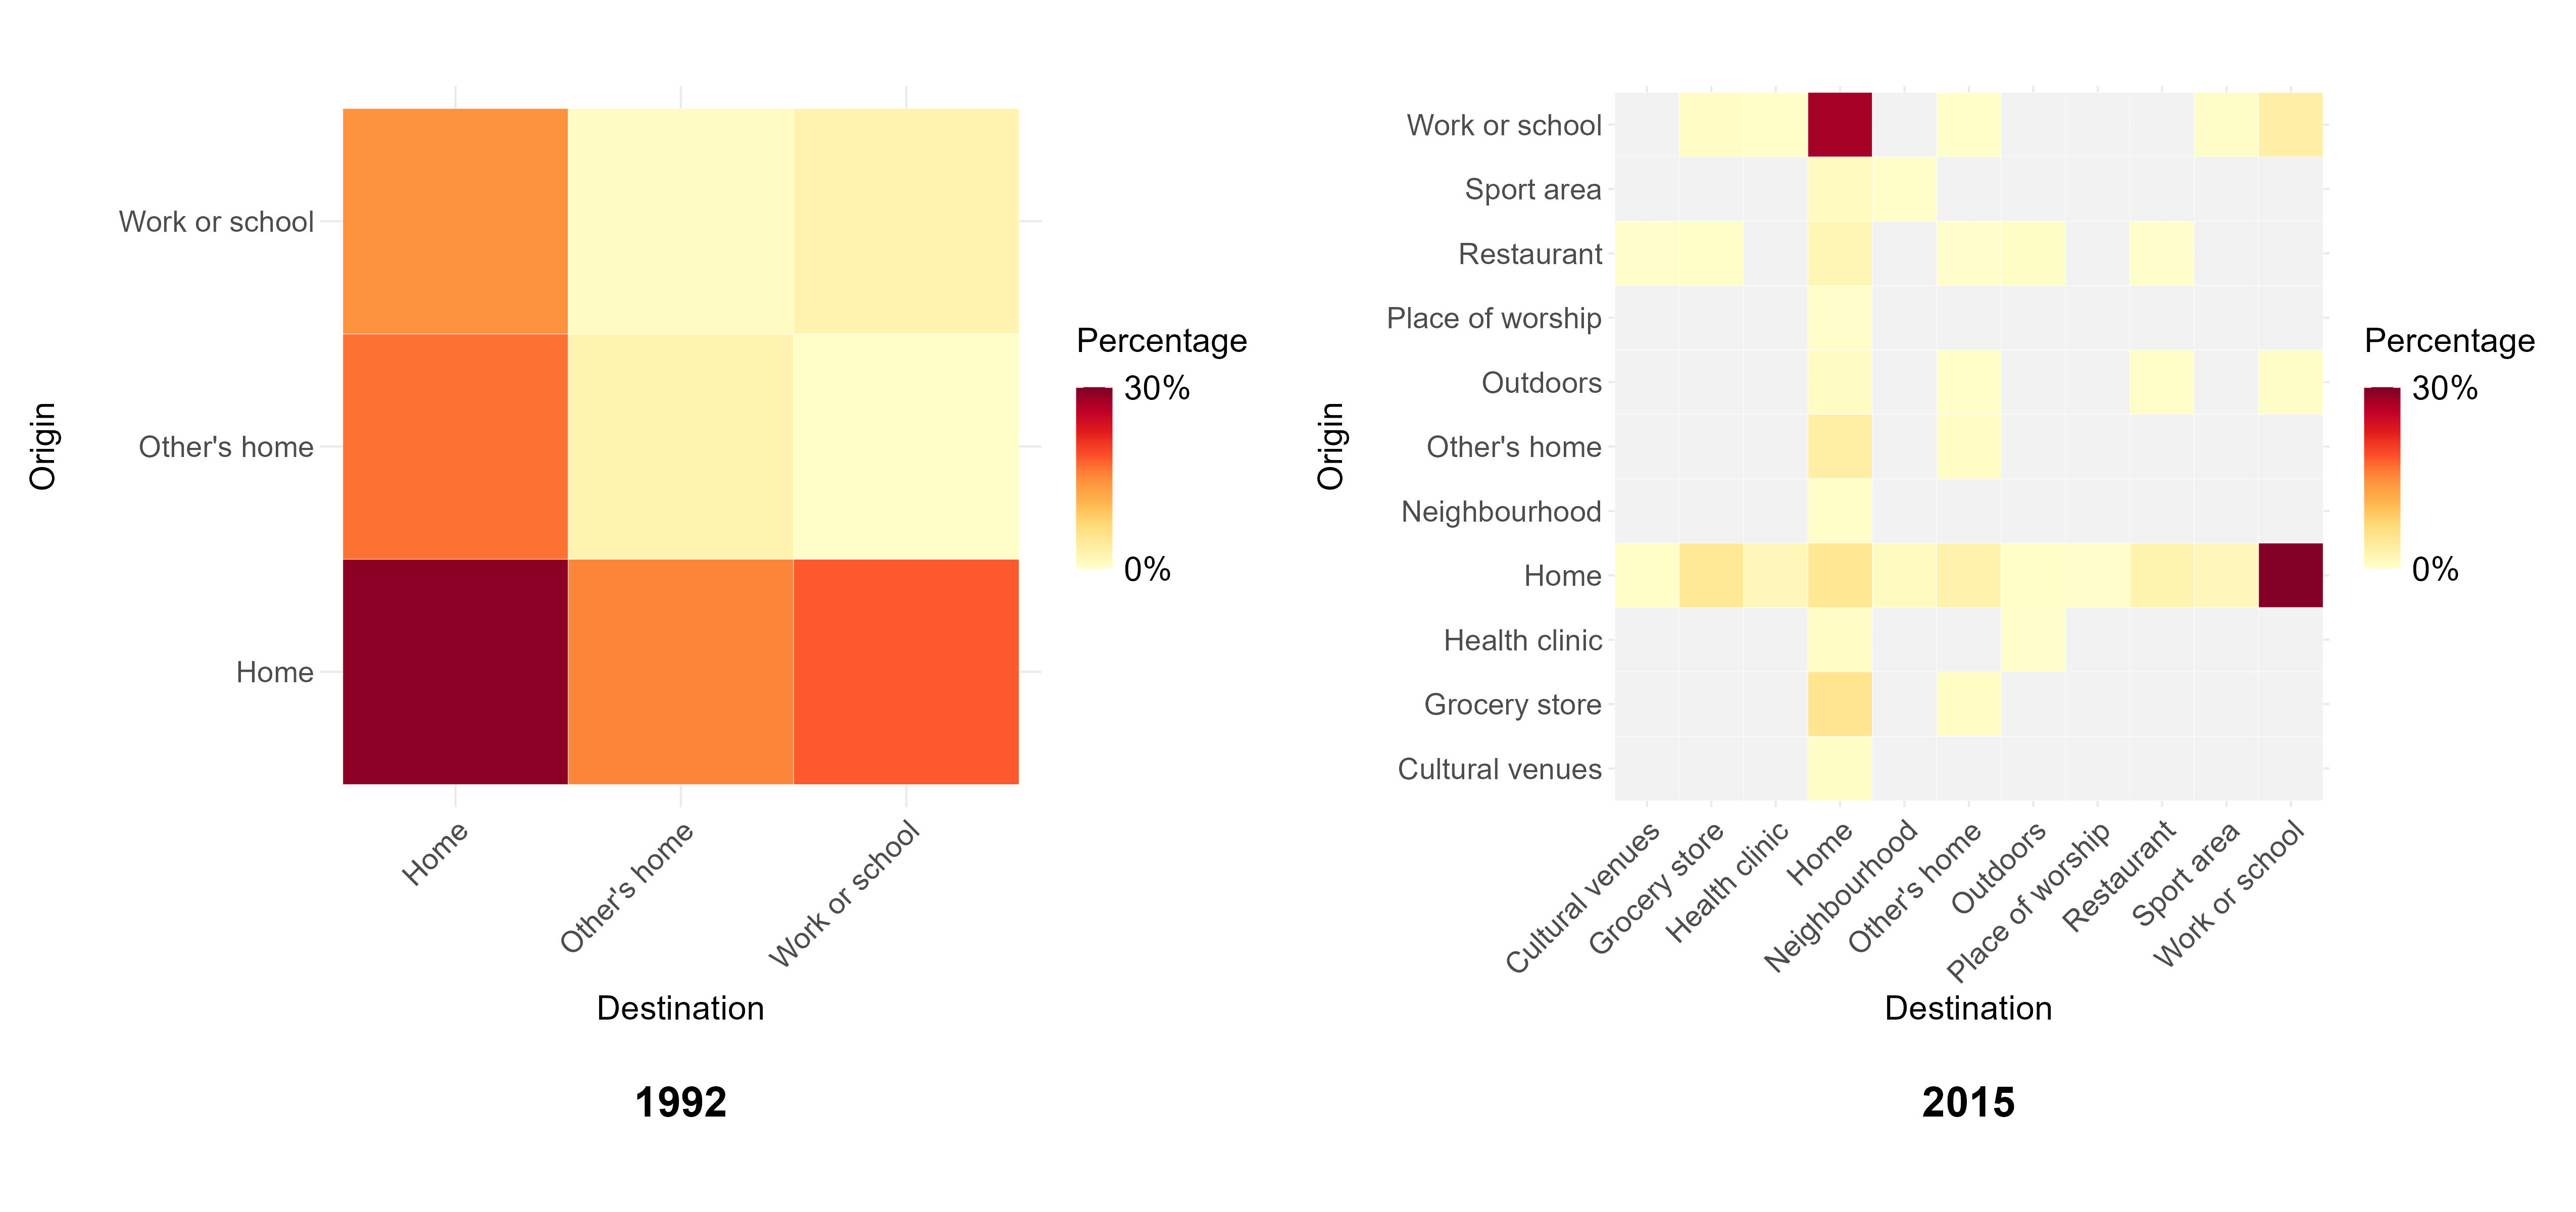
\includegraphics[width=1\linewidth]{Manuscript-figures/cycling_hm_fig} 

}

\caption{Percentage of walking Trips Categorized by Origin and Destination}\label{fig:figure-02}
\end{figure}

\hypertarget{impedance-functions-for-canadians-metropolitan-and-census-agglomerations-areas}{%
\section{Impedance functions for Canadians Metropolitan and Census
Agglomerations
areas}\label{impedance-functions-for-canadians-metropolitan-and-census-agglomerations-areas}}

Impedance functions reveals important information about the travel
behavior of the population, by describing the relationship between the
population at an origin and their likelihood or ability to travel to
specific destinations to access opportunities \citep{soukhov2024}.

Impedance functions are commonly used in accessibility analysis to
calculate the cost of travel between different locations
\citep{hansen1959, páez2012, palacios2022}. However, these functions
need to be calibrated in order to accurately represent travel behavior.
One effective way of calibrating an impedance function is by using the
trip length distribution (TLD) obtained from origin-destination data
\citep{soukhov2024}. The TLD represents the probability that a certain
proportion of trips will be made at a specific cost, such as travel
time. In this data set, low travel times are associated with a higher
proportion of trips, while high travel times are associated with a lower
proportion of trips.

\{ActiveCA\} provides calibrated impedance functions for Canadian
Metropolitan and Census Agglomeration areas. For each combination of
year, destination, and transportation mode, we fitted the most suitable
impedance function based on empirical data from the GSS surveys.
\{ActiveCA\} includes a total of 64 distance-decay functions. These were
estimated using the \texttt{fitdistrplus} package
\citep{mullerdutang2015}, selecting the distribution with the lowest
Akaike information criterion (AIC) among exponential, gamma, log-normal,
normal, and uniform types.

Table \ref{tab:table-04} shows the best impedance functions for walking
trips to \texttt{Work\ or\ school} across survey years, where all
distributions, except for a gamma function in 1998, are log-normal.
Figure \ref{fig:figure-03} illustrates these fitted functions (red line)
alongside histograms of empirical travel times (grey bars). As for the
others functions, these examples enable to calculate gravity-based
accessibility measures for active transportation modes across various
destinations and temporal scales in Canadian urban areas.

\begin{table}
\centering
\caption{\label{tab:table-04}\label{table-04}Impedance functions and AIC for `Walking` trips considering `Work or school` as destination.}
\centering
\resizebox{\ifdim\width>\linewidth\linewidth\else\width\fi}{!}{
\fontsize{10}{12}\selectfont
\begin{threeparttable}
\begin{tabular}[t]{rlrrr}
\toprule
\multicolumn{1}{c}{\textbf{Year}} & \multicolumn{1}{c}{\textbf{Impedance function*}} & \multicolumn{1}{c}{\textbf{Parameter 1*}} & \multicolumn{1}{c}{\textbf{Parameter 2*}} & \multicolumn{1}{c}{\textbf{AIC}}\\
\midrule
2015 & lnorm & 2.55 & 0.64 & 6612061\\
2010 & lnorm & 2.21 & 0.78 & 7917431\\
2005 & lnorm & 2.13 & 0.79 & 8182691\\
1998 & gamma & 1.23 & 0.09 & 2318752\\
1992 & lnorm & 2.38 & 0.70 & 2319400\\
\bottomrule
\end{tabular}
\begin{tablenotes}
\item \textit{Note: } 
\item * `lnorm` refers to the log-normal distribution. For `lnorm` distributions, `Parameter 1` and `Parameter 2` refer to the mean and standard deviation of the distribution on the logarithmic scaler, respectively. For the `gamma` distribution, `Parameter 1` and `Parameter 2` refer to the rate and shape of the distribution, respectively. `AIC` means Akaike information criterion.
\end{tablenotes}
\end{threeparttable}}
\end{table}

\begin{figure}

{\centering 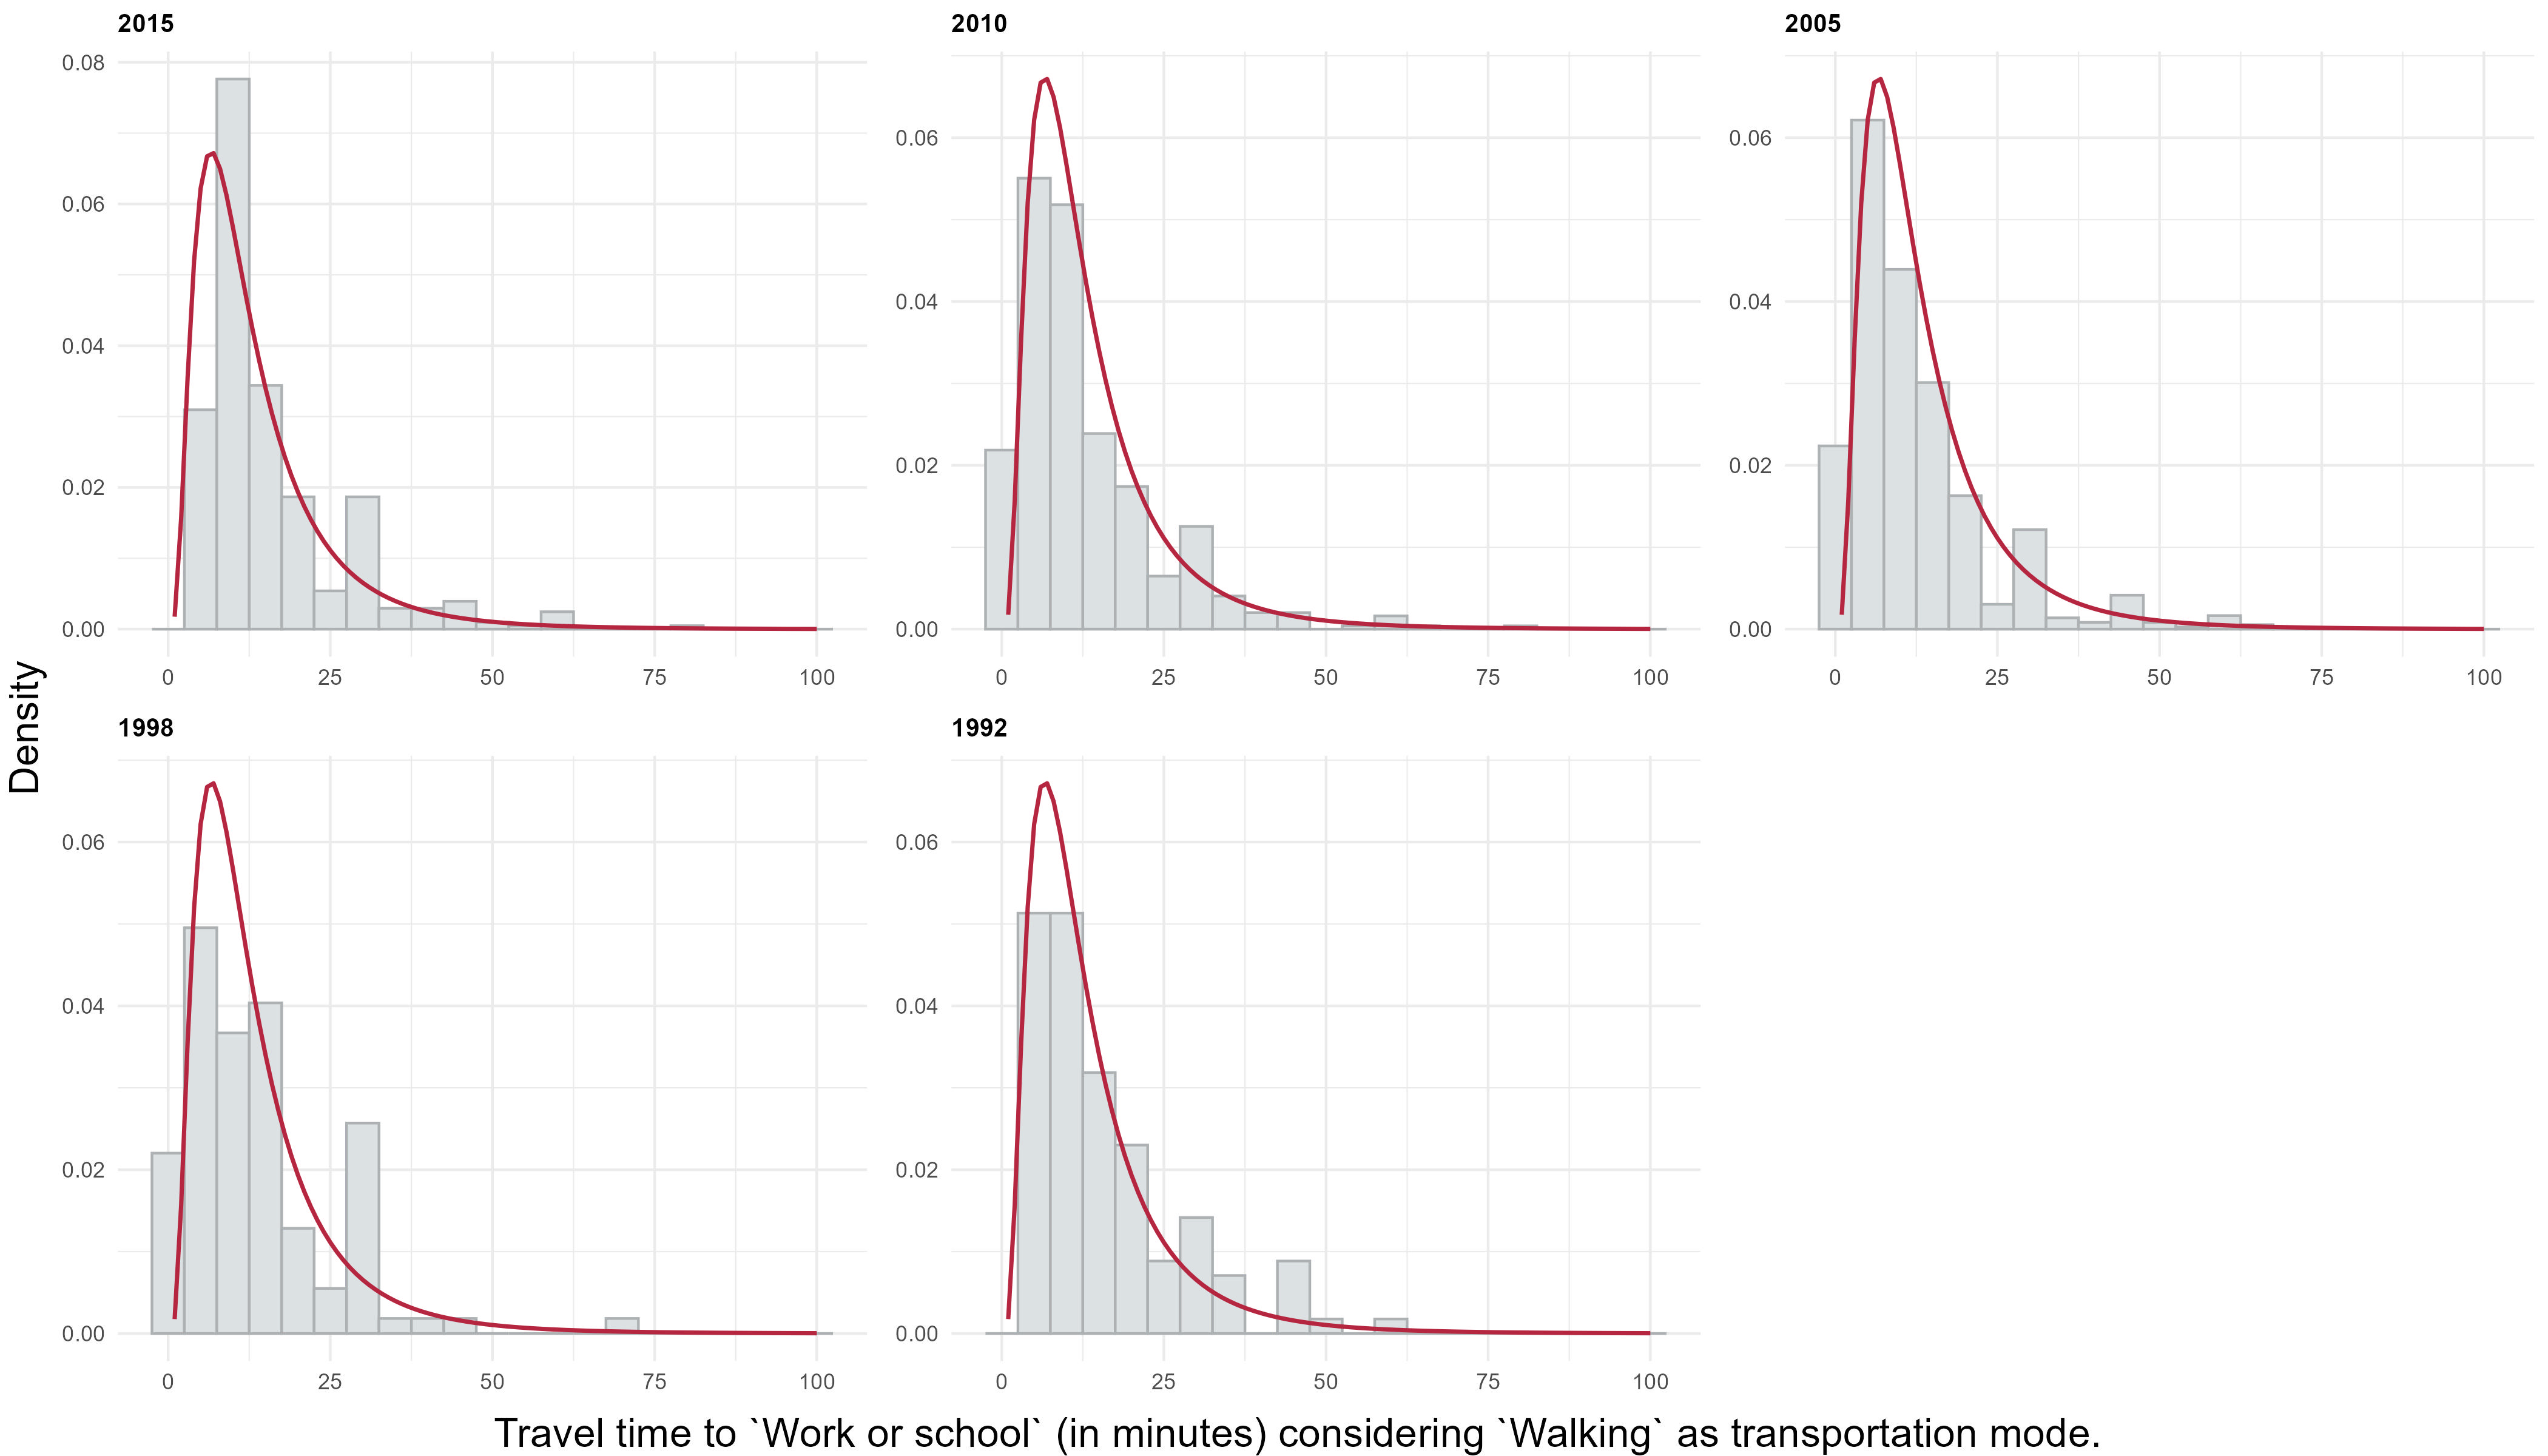
\includegraphics[width=1\linewidth]{Manuscript-figures/impf_Work or school_Walking} 

}

\caption{Percentage of walking Trips Categorized by Origin and DestinationWalking}\label{fig:figure-03}
\end{figure}

\hypertarget{concluding-remarks}{%
\section{Concluding remarks}\label{concluding-remarks}}

This article introduces \{ActiveCA\}, an open data product in the form
of an R data package, developed after the collection, cleaning, and
processing of General Social Survey data ranging from 1986 to 2015. The
package provides analysis-ready data on active transportation episodes,
focusing on walking and cycling activities, with information on trip
origins, destinations, and duration. Additionally, the package includes
a series of impedance functions calibrated for various destinations,
considering the different transportation modes and time periods.

The value of \{ActiveCA\} lies in its transparency, accessibility, and
open infrastructure, which facilitates the addition of complementary
data sets in the future. R users can seamlessly explore GSS walking and
cycling episodes along with calibrated impedance functions, with the
option to suggest enhancements to the package as needed. This article
adopts the structure proposed by Anastasia and Páez
\citeyearpar{soukhov2023}, whose work provided essential guidance for
the creation of this package. Similarly, we aim to contribute to the
academic community by promoting transparent research practices that
encourage replication and innovation in related fields. We believe that
\{ActiveCA\} will serve as a basis for further research on GSS and for
the integration of additional data by the authors or the wider open
source community.

\hypertarget{declaration-of-conflicting-interests}{%
\section{Declaration of Conflicting
Interests}\label{declaration-of-conflicting-interests}}

The author(s) declared no potential conflicts of interest with respect
to the research, authorship, and/or publication of this article.

\hypertarget{funding}{%
\section{Funding}\label{funding}}

The author(s) disclosed receipt of the following financial support for
the research, authorship, and/or publication of this article: This work
was supported by the Social Sciences and Humanities Research Council of
Canada (\emph{More description about the funding source after the review
process}).

\hypertarget{orcid}{%
\section{ORCID}\label{orcid}}

Author 1 Author 2 Author 3

\hypertarget{data-availability-statement}{%
\section{Data availability
statement}\label{data-availability-statement}}

The \{ActiceCA\} R data package can be found and installed on Github
(\emph{link}).

\bibliographystyle{sageh}
\bibliography{bibfile.bib}


\end{document}
